\chapter{Analysis}

Before going over the actual programming of the framework, we need to further inspect some of the features we have specified in the Introduction in Chapter \ref{Intro}. In this chapter, we will analyse features of this project, as well as suggest ways of solving problems, and in case there are more solutions, we will select the most suitable one with a proper explanation.

\section{Command System}


\section{Walking system}
In Requirement \ref{intro:req:pathfinding}  we have established that the player should have the ability to move around the playable area (map). The development of the walking system could be divided into two main parts:
\begin{enumerate}
    \item The representation of the walkable area,
    \item The problem of finding the path to a goal.
\end{enumerate} 

\subsection{Walkable Area}
\label{analysis:walkableMap}

The characters in a video game exist within a defined in-game world. Naturally, this world needs boundaries and areas where the player can move and interact. The walkable area refers to the regions of the game world that the player is allowed to access and navigate. It often consists of a collection of rooms, but it could be just as easily a city square, a forest, or any other kind of space that the developer envisions. While it is easy to imagine these spaces and the areas accessible to the player in our minds, we need a clear and practical way to define them within the game engine. 

\subsubsection{Bitmap}
In his article, Steven Henk Don \cite{Shdon} outlines an approach to representing walkable areas using a walkability bitmap. This method involves creating an image composed of a limited set of colors, where each color conveys specific information about the game environment. In our case, this bitmap would describe the possible walkable areas that the player may traverse. Figure \ref{fig:WS:Bitmap} shows one such bitmap on top of the scene. In this example, the player is able to freely walk around the area highlighted with green color, while the dark areas are inaccessible. Finally, the player can step on the blue area only when certain conditions are met (e.g. after talking to the bouncer).  

\begin{figure}[H]
\centering
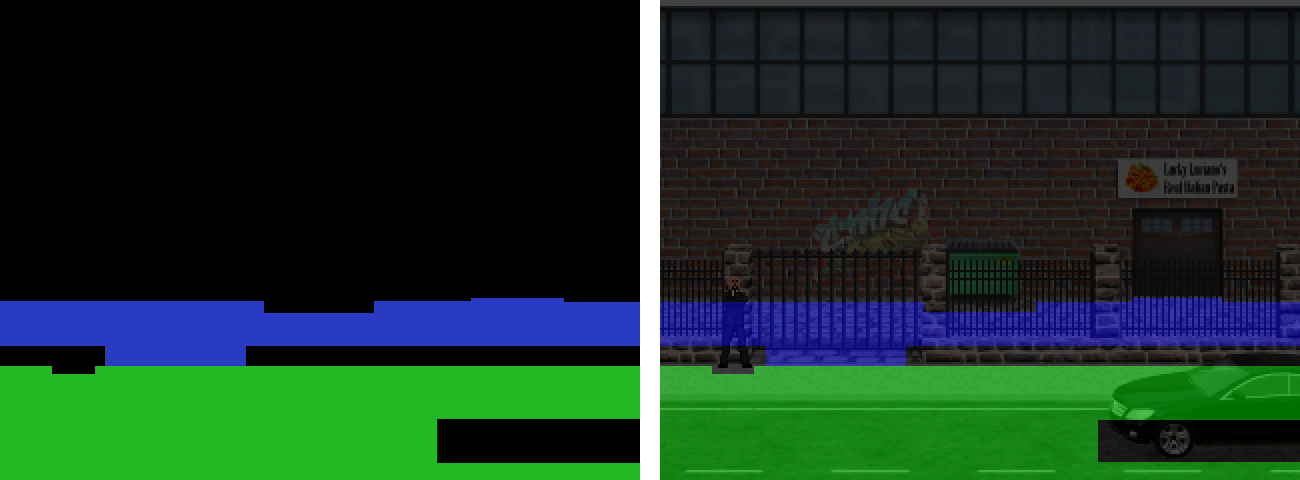
\includegraphics[width=1.0\linewidth]{img/walkability-map2.png}
\caption{Walkability bitmap: bitmap mask (left) and mask applied on top of a scene (right). Source \cite{Shdon}.}
\label{fig:WS:Bitmap}
\end{figure}

To obtain such a bitmap, the user must use image-editing software to manually create colorful shapes that represent the accessible parts of the environment and then save the image. Additionally, modifying the bitmap is difficult and time-consuming, as it requires reopening the editing software and making manual changes. Our goal is to find a solution that can be integrated directly into the framework while keeping the experience user-friendly, something this approach does not support. 

\subsubsection{Polygons}
Another approach to this problem is discussed in detail in articles by Mic Uurloon \cite{Uurloon1}\cite{Uurloon2}, where walkable areas and obstacles are defined using polygon shapes directly within the Unity engine. The idea is to have one primary shape that defines the main walkable area, be it a room, a hall, or a town square. Inside that area, there can be places that are not accessible currently or indefinitely (e.g. furniture), let us call them obstacles. We can define the boundaries of the walkable area and the obstacles using polygons, as seen in Figure \ref{fig:WS:Poly}. One such polygon can be used to outline the primary area where the user walks around, while additional polygons can be viewed as obstacles that the player must avoid.

\begin{figure}[H]
\centering
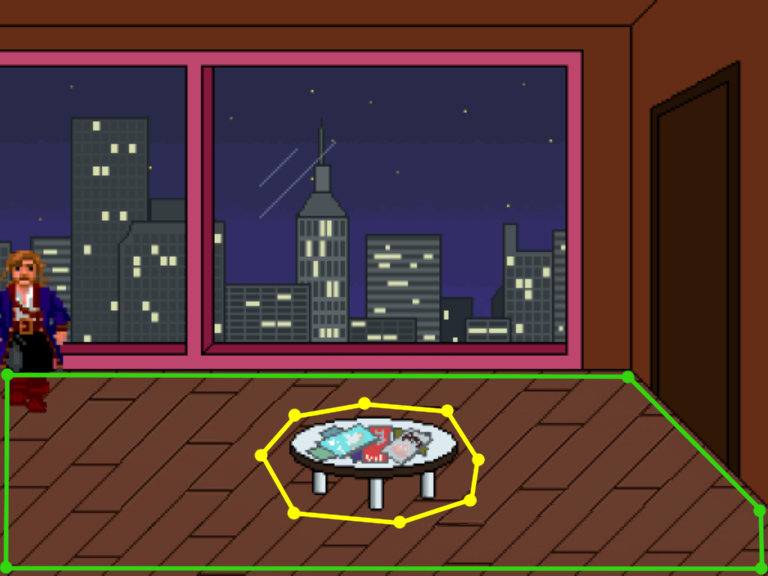
\includegraphics[width=.7\linewidth]{img/WS-polygons4.png}
\caption{Polygonal map: the room as the main walkable area (green) and the table as an obstacle (yellow). Source \cite{Uurloon1}.}
\label{fig:WS:Poly}
\end{figure}

The main advantage of this approach is the ability of the user of the framework to modify the shapes on the fly whenever necessary. Next, this system can be implemented directly in Unity and does not require any other software to set it up. For these reasons, we decided to go with this solution.

\subsubsection{Sierra}
Since Chapter \ref{Intro} focused heavily on the features of classic point-and-click games, it makes sense to now examine how walking systems are implemented by prominent studios. Unfortunately, there is limited publicly available information on this topic, possibly due to the existence of patents or proprietary techniques that are not openly shared. However, we have found one notable example. According to ScummVM, an open-source project that reimplements classic game engines, a prominent game company Sierra behind classics such as \textit{King's Quest} implemented their own patented pathfinding algorithm designed to navigate game characters around obstacles \cite{ScummVM-polygons}. Similarly to the second approach, it uses polygons to represent the area as well as the obstacles. But unlike it, is also uses a complex system of four types of polygons with different rules. 
\begin{itemize}
    \item  \textit{Barred access polygons} strictly block entry, meaning if the end point lies inside one, the path ends at the nearest point on the polygon’s boundary. 
    \item On the other hand, \textit{total access polygons} are ignored if the start or end point is inside them, allowing paths to begin or end there, but otherwise preventing entry. \textit{
    \item Near-point access polygons} require that the path enters or exits through the closest boundary point (near-point) if the start or end lies within. 
    \item Finally, \textit{contained access polygons} define strict boundaries within which the entire path must remain; if the end point lies outside, the path stops at the near-point. Since polygons cannot intersect, only one contained access polygon can exist in a scene.
\end{itemize}

This method is very similar to the one introduced in the previous section but with more options to allow...

\subsection{Pathfinding}
A crucial part of character movement is the ability to find a path to the goal. The simplest option is to take a direct line to the goal. However, this approach drastically restricts the types of map available. Firstly, the main walkable area is only restricted to basic shapes like triangles, rectangles, and squares, where any two points can be connected by a straight line that is entirely contained inside that shape. However, if the walkable area is concave (containing one or more concave verices), some vertices point inward, creating obstructions that block direct visibility between points, as depicted in Figure \ref{fig:Polygons}.

\begin{figure}[H]
\centering
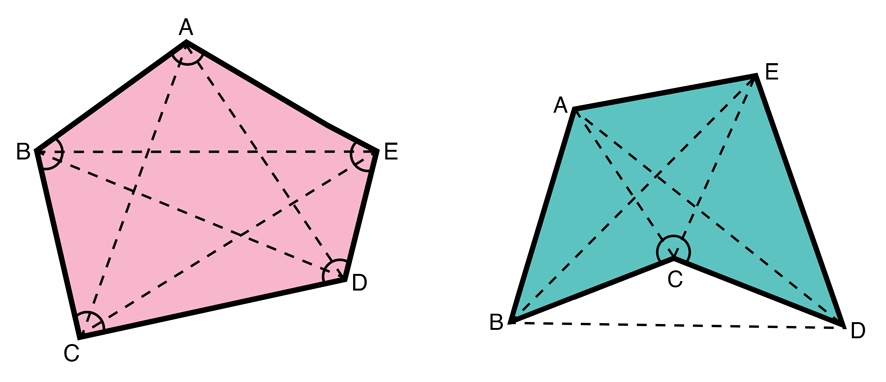
\includegraphics[width=.8\linewidth]{img/polygons.png}
\caption{Convex (left) and concave (right) polygons. Source \cite{Polygons}.}
\label{fig:Polygons}
\end{figure}

But it is not just the shape of the main walkable area that poses limitations. The idea of placing obstacles within that area introduces a challenge, as a straight line alone cannot accurately represent the action of navigating around such objects. This means that areas like the ones in Figures \ref{fig:Path-B}  and \ref{fig:Path-M}  cannot be replicated.

\begin{figure}[H]
\centering
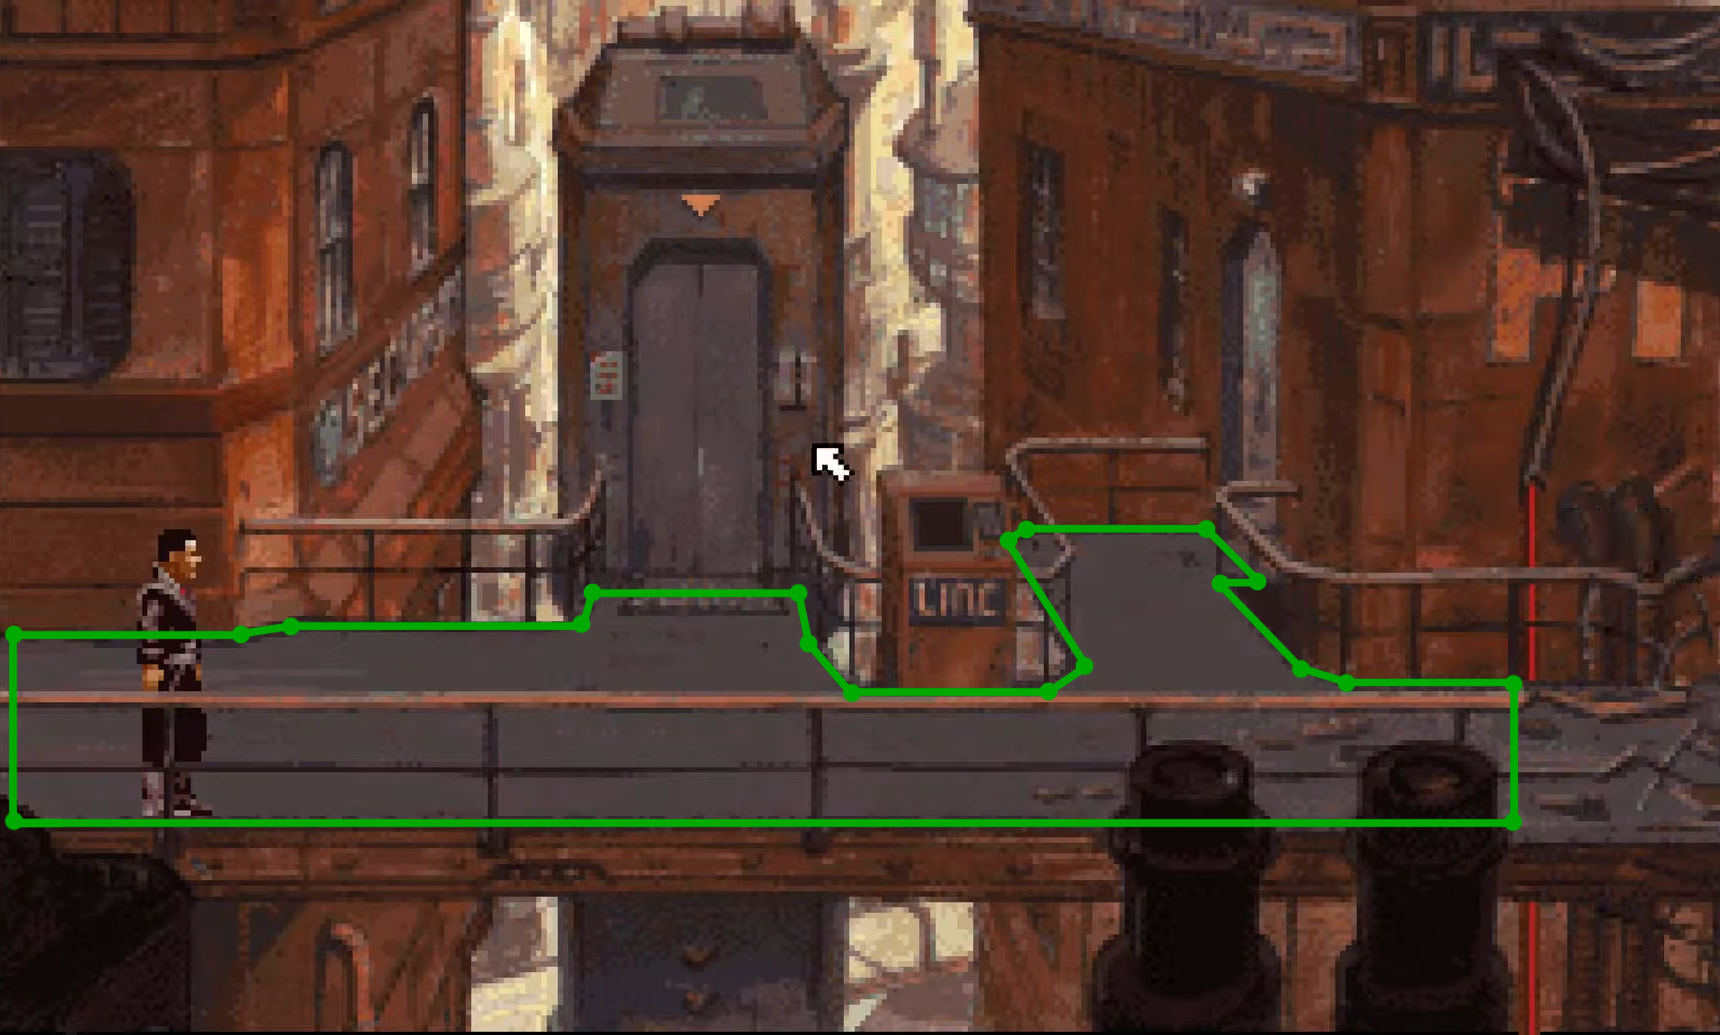
\includegraphics[width=.7\linewidth]{img/Path-BaSS.png}
\caption{Beneath a Steel Sky: A concave path where no one straight line would access each point from where the character is standing.}
\label{fig:Path-B}
\end{figure}

\begin{figure}[H]
\centering
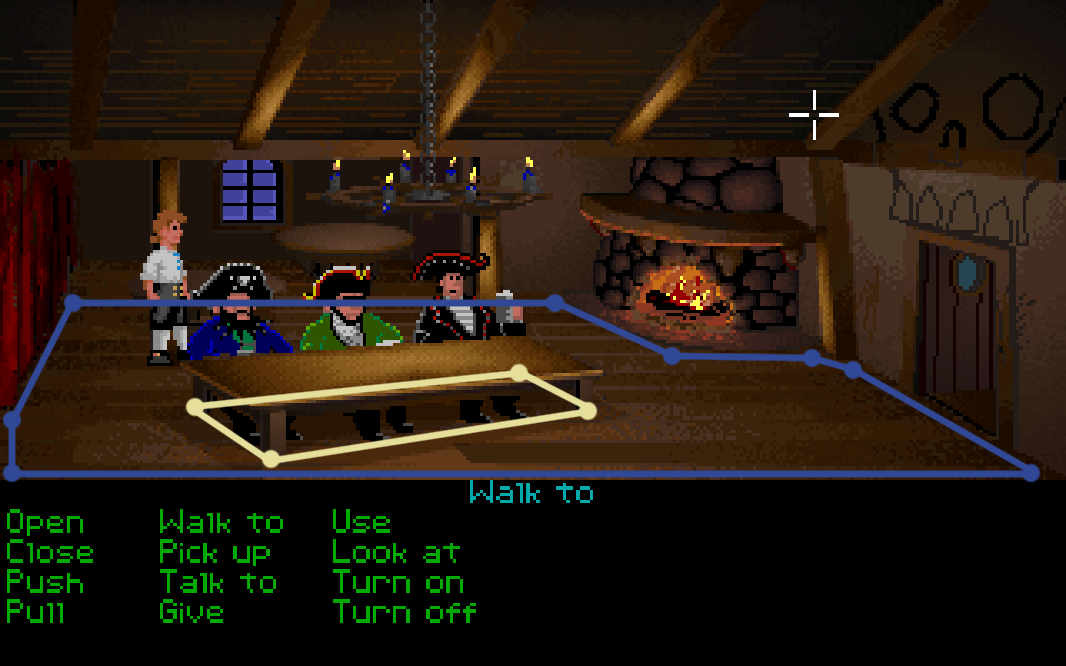
\includegraphics[width=.7\linewidth]{img/Path-TSoMI.png}
\caption{The Secret of Monkey Island: An obstacle (table) in the middle of the room restricts the player's access to the other part of the room.}
\label{fig:Path-M}
\end{figure}

So if one straight line is not enough, we can use multiple lines. This way of dividing the path into smaller sub-paths allows the character to get to the goal while being restricted to the walkable area. But now the question is which lines we should chose.

We might intuitively imagine an algorithm that first attempts to follow a straight line toward the goal. When an obstacle approaches, whether it is the edge of the walkable area or an internal obstacle, it would try to move sideways and find a way around it. While this seems like a reasonable approach, it does not truly solve the core problem: finding an actual route. Instead, it merely postpones the decision-making. So what are our options?

A naive strategy would be to follow the edge of the obstacle, either to the left or to the right, until a straight line to the goal becomes possible again. If another obstacle is encountered, the process repeats. However, this approach glosses over a critical point: How do we decide which direction to follow? Picking a random direction can lead to highly inefficient paths. The Figure \ref{fig:Path-P}  highlights a situation where the goal is to get to the right side of the polygon. However, the direct path (blue) is obstructed by an edge of the polygon itself. Looking at the picture, we can see that following red path on the left causes an unnecessary detour, making the movement appear unnatural. Ideally, we want the path to look natural and intuitive, similar to the green path to the right.

\begin{figure}[H]
\centering
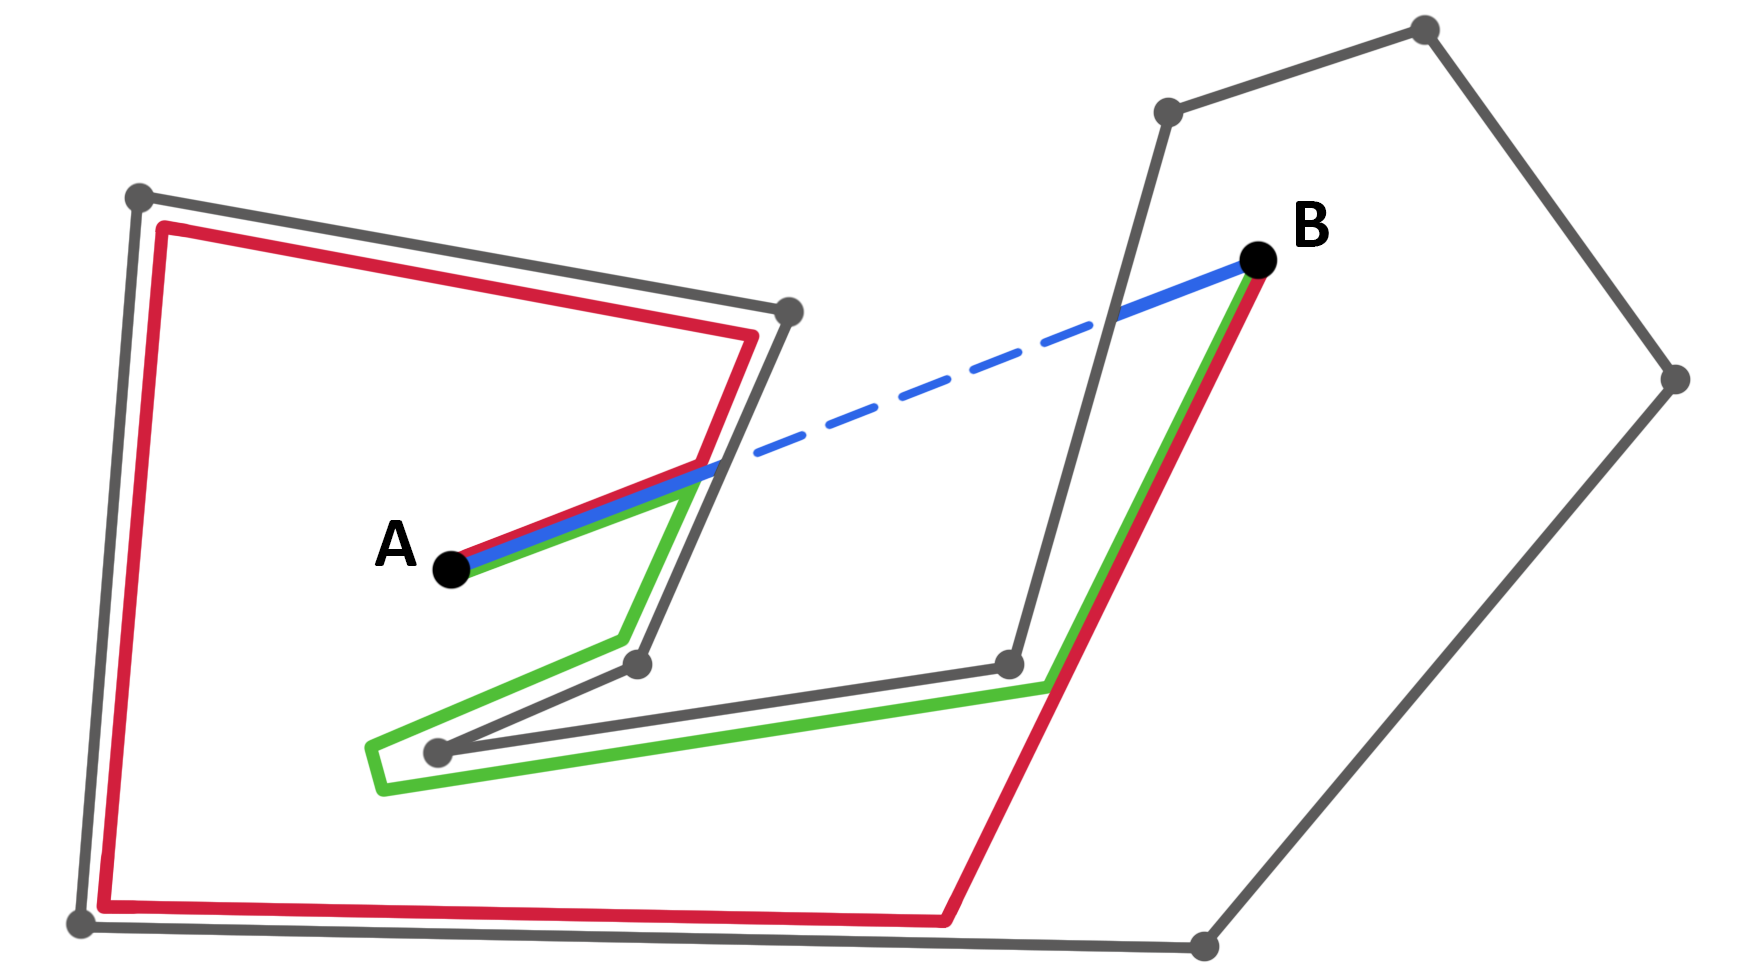
\includegraphics[width=.7\linewidth]{img/polygon-prototyp.png}
\caption{Pathfinding in a concave polygon - simple approach}
\label{fig:Path-P}
\end{figure}

In real life, people instinctively aim for the shortest or most efficient route. By comparing the left and right paths in Figure \ref{fig:Path-P}, we can identify the shorter one - likely the more natural and visually appealing choice. But even this can be improved. If we examine the start of the path, our algorithm initially attempts to move straight toward the goal until hitting an obstacle. However, a person would probably try to avoid the obstacle from the beginning, aiming to take the shortest path right away. That’s the key insight: instead of reacting to obstacles as they come, we should aim to find the shortest path from the start, just like the one in Figure \ref{fig:Path-P2}.
 
\begin{figure}[H]
\centering
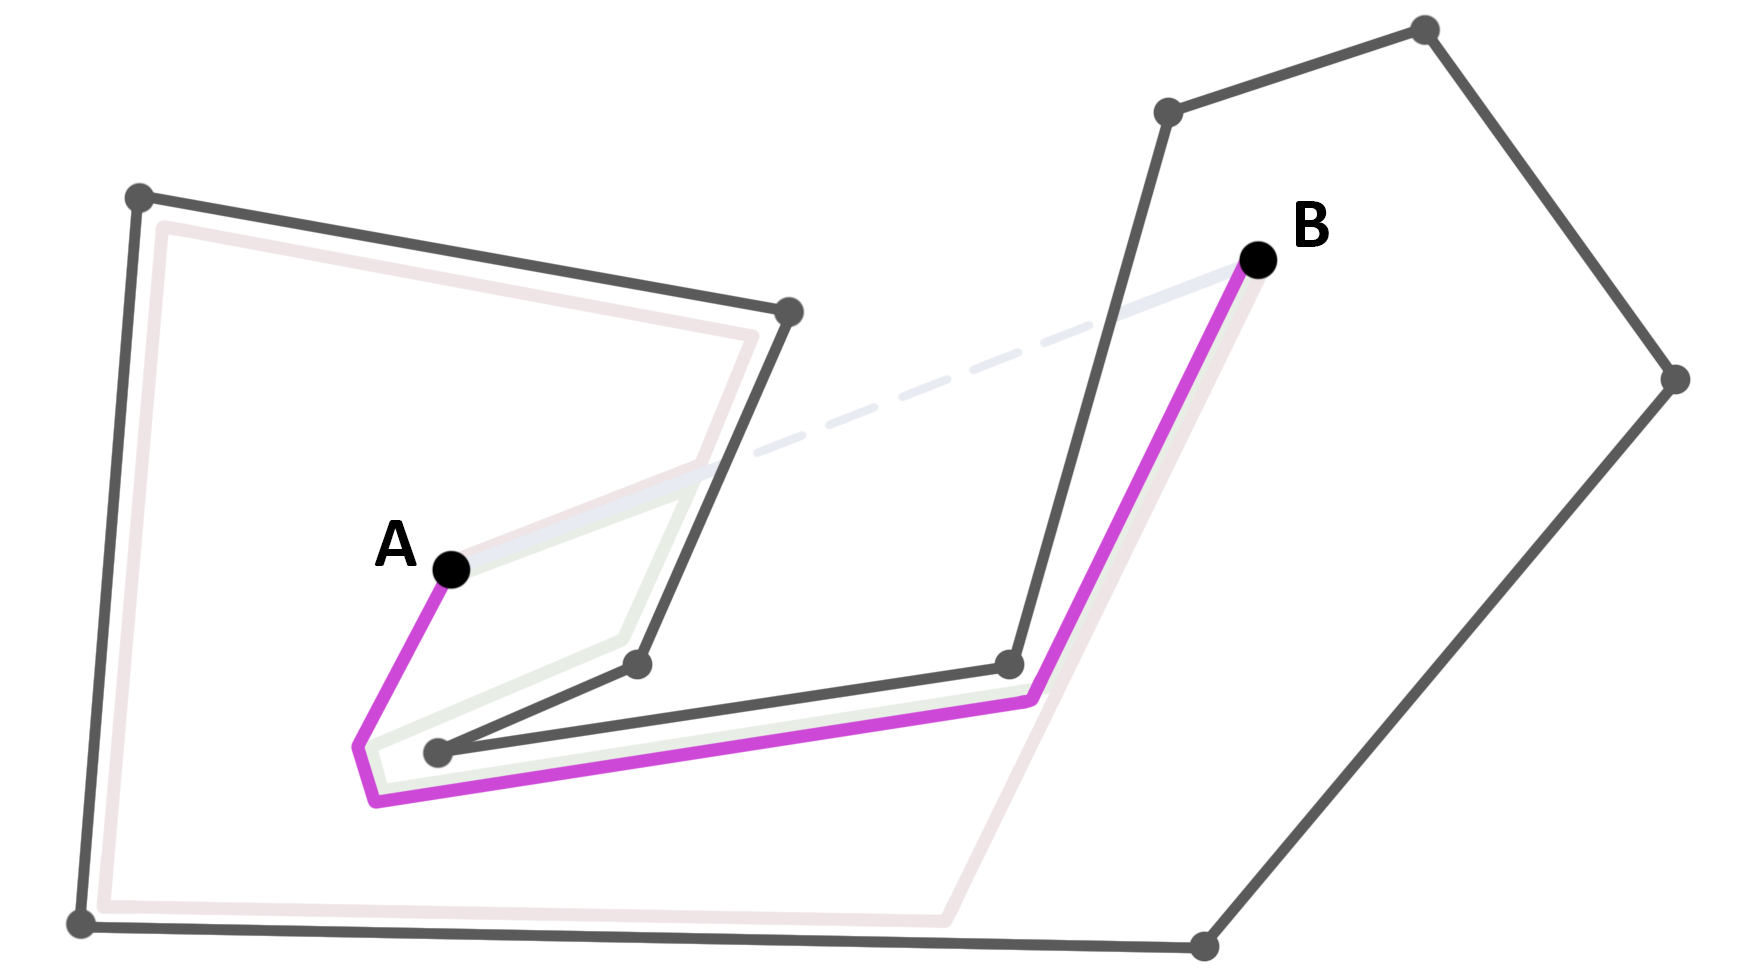
\includegraphics[width=.7\linewidth]{img/polygon-prototyp2.png}
\caption{Pathfinding in a concave polygon - shortest path}
\label{fig:Path-P2}
\end{figure}

A very similar approach was also used in Sierra's engine with multiple levels of optimization that essentially aim to find the shortest path to the goal \cite{ScummVM-patent}.


%Objects typically get there by taking the shortest route possible. This makes sense in point-and-click adventure games, as player input is intentional and direct: clicking on a location implies that the character should move there efficiently, without unnecessary detours. The problem of finding the shortest path is a well-studied field in computer science, with several established algorithms designed to solve it. 

\subsubsection{Weighted Graph}
Polygons only serve as a visual representation of the walkable area to the framework users, and essentially this is everything they need to care about. However, to enable algorithms like pathfinding to operate effectively, the walkable area must also be represented in a form suitable for computation. Specifically, if we want to determine the shortest path to a destination, we need a way to calculate the distances between the points—without this, identifying the optimal route would be impossible. A weighted graph provides an ideal structure for this purpose. It consists of nodes connected by edges, each assigned a non-negative value representing the distance between them. That said, generating a graph that includes every possible node and edge would be both inefficient and impractical. The approach for creating a graph from polygons that was used in our project was adapted from the articles by Mic Uurloon. Details about this method together with more interactive examples explaining how the algorithm works can be found in his articles Part 1 \cite{Uurloon1} and Part 2 \cite{Uurloon2}, which further reference an article by David Gouveia \cite{Gouveia}.

So let us set up some rules that we need to follow:

\begin{enumerate}[label=\color{purple}\textbf{R{\arabic*}}]
  \item \label{analysis:concave} In the main polygon, every concave vertex (a vertex with an interior angle greater than 180°) is a node.
  \item \label{analysis:convex} In the obstacle polygons, every convex vertex (a vertex with an interior angle less than 180°) is a node.
  \item \label{analysis:start} The position of the character (start position) is a node.
  \item \label{analysis:end} The end position (e.g. the mouse cursor) is a node.
  \item \label{analysis:LOS} For each two nodes, we create an edge if they are in line of sight (a straight line from a node to another node inside the polygon without crossing an edge of any polygon). 
\end{enumerate}

According to Rule \ref{analysis:concave}, a node is included based on type of the vertex of the corresponding polygon. In basic shapes like triangles, rectangles, and squares, any two points can be connected by a straight line without encountering obstacles. However, if the walkable area is concave (containing one or more concave verices), some vertices point inward, creating obstructions that block direct visibility between points, as depicted in Figure \ref{fig:Polygons}. To account for these obstructions, a node is added to the graph only if its corresponding vertex is concave. On the other hand, convex vertices are excluded as they do not create such obstructions.


To determine which vertices are convex, we can iterate through them one by one and check the angle formed by the lines from the previous and next vertices to the current one. We do that by calculating the cross product, as seen in Algorithm \ref{alg:IsVertexConcave}.

\algrenewcommand\algorithmicrequire{\textbf{Input:}}
\algrenewcommand\algorithmicensure{\textbf{Output:}}
\renewcommand{\alglinenumber}[1]{#1.}  % Change numbering from "1:" to "1."
\begin{algorithm}[H]
\caption{Check if a Vertex is Concave}\label{alg:IsVertexConcave}
\begin{algorithmic}[1]
\Require Array of vertices $vertices$, index of vertex $vertex$
\Ensure \textbf{true} if the vertex is concave, \textbf{false} otherwise
\Statex
\Function{IsVertexConcave}{$vertices, vertex$}
    \State $current \gets vertices[vertex]$
    \State $next \gets vertices[(vertex + 1) \bmod \Call{Length}{vertices}]$
    \If{$vertex = 0$}
        \State $previous \gets vertices[\Call{Length}{vertices} - 1]$
    \Else
        \State $previous \gets vertices[vertex - 1]$
    \EndIf
    \State $left \gets$ \Call{Vector}{$current.x - previous.x,\ current.y - previous.y$}
    \State $right \gets$ \Call{Vector}{$next.x - current.x,\ next.y - current.y$}
    \State $cross \gets (left.x \cdot right.y) - (left.y \cdot right.x)$
    \State \Return $cross < 0$
\EndFunction
\end{algorithmic}
\end{algorithm}

However, this method can produce incorrect results if the vertex order is not handled carefully. Reversing the order of the vertices results in the opposite angle, which may misclassify the convex and concave points (see Figure \ref{fig:Clock}). The Algorithm \ref{alg:IsVertexConcave} works only in the case that the vertices of a polygon are ordered clockwise. To avoid getting the wrong result, we must also check that the vertices are ordered clockwise or counter-clockwise. This can be done using the Algorithm \ref{alg:IsOrientationClockwise}.
The algorithm essentially calculates a signed value based on the positions of consecutive vertices. It does this by summing the expression $(b.x-a.x)\cdot(b.y+a.y)$ for each edge, where $a$ and $b$ are adjacent vertices. A positive result indicates a clockwise orientation, while a negative result indicates counter-clockwise.

\begin{figure}[H]
\centering
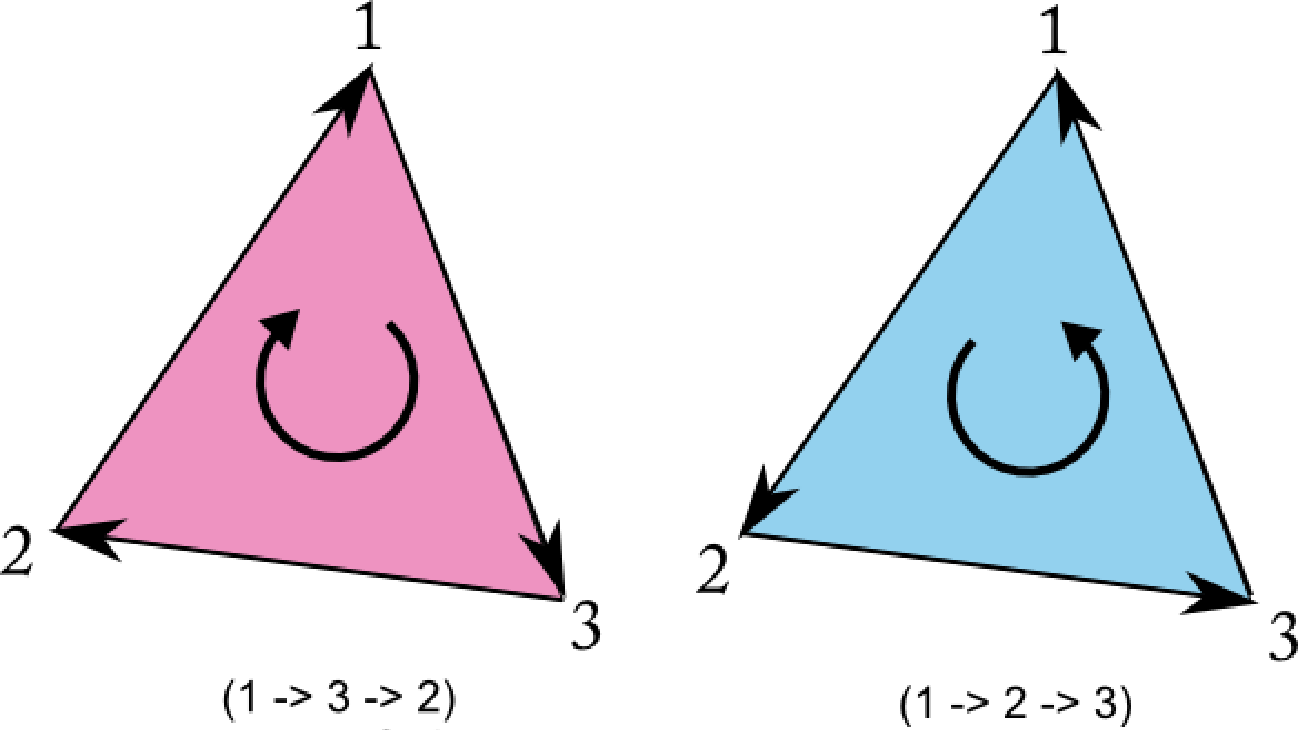
\includegraphics[width=.6\linewidth]{img/clock.png}
\caption{Clockwise (left) and counter-clockwise (right) polygons. Source \cite{Clock}.}
\label{fig:Clock}
\end{figure}

\begin{algorithm}[H]
\caption{Check if Polygon Orientation is Clockwise}\label{alg:IsOrientationClockwise}
\begin{algorithmic}[1]
\Require Array of vertices $vertices$
\Ensure \textbf{true} if orientation is clockwise, \textbf{false} otherwise
\Statex
\Function{IsOrientationClockwise}{$vertices$}
    \State $sum \gets 0$
    \For{$i \gets 0$ to $\Call{Length}{vertices} - 1$}
        \State $a \gets vertices[i]$
        \State $b \gets vertices[(i + 1) \bmod \Call{Length}{vertices}]$
        \State $sum \gets sum + (b.x - a.x) \cdot (b.y + a.y)$
    \EndFor
    \State \Return $sum > 0$
\EndFunction
\end{algorithmic}
\end{algorithm}

The next rule \ref{analysis:convex} tells us that the situation is reversed for obstacles (meaning non-main polygons) as we do not want to stay inside these obstacles but on the outside. Since we need to go around them, in this case we include convex vertices instead of concave ones. Here, the concave vertices do not stand in the way of two points, but the convex ones do. 

When it comes to the starting and ending positions (typically those of the main character and the mouse cursor), we need to include them as well. Because our primary aim is to find a path between them in the graph, the Rules \ref{analysis:start} and \ref{analysis:end} are necessary for this purpose.

Finally, in terms of edges, an edge is included in the graph only if the two nodes that form it are within each other's line of sight, as mentioned in Rule \ref{analysis:LOS}. If other edges were included, we would get edges that run through obstacles and outside of the main walkable area, which is definitely not what we want. This is why we need to do a check of visibility. The Algorithm \ref{alg:InLineOfSight} depicts the process of check if two nodes are in line of sight. \todo{finish this}

\begin{algorithm}
\caption{Check Line of Sight Between Two Points}\label{alg:InLineOfSight}
\begin{algorithmic}[1]
\Require Start point \texttt{start}, End point \texttt{end}, List of polygons \texttt{polygons}
\Ensure \textbf{true} if \texttt{start} and \texttt{end} are in line of sight, \textbf{false} otherwise
\Statex
\Function{InLineOfSight}{start, end}
    \State $\epsilon \gets 0.5$
    \If{not polygons[0].pointInside(start) or not polygons[0].pointInside(end)}
        \State \Return \textbf{false}
    \EndIf
    \If{Length(Subtract(start, end)) < epsilon}
        \State \Return \textbf{false}
    \EndIf
    \State inSight $\gets$ \textbf{true}
    \ForAll{polygon in polygons}
        \For{$i \gets 0$ to Length(polygon.vertices) $-1$}
            \State $v1 \gets$ polygon.vertices[$i$]
            \State $v2 \gets$ polygon.vertices[$(i+1) \bmod$ Length(polygon.vertices)]
            \If{LineSegmentsCross(start, end, v1, v2)}
                \If{distanceToSegment(start.x, start.y, v1.x, v1.y, v2.x, v2.y) > 0.5 and distanceToSegment(end.x, end.y, v1.x, v1.y, v2.x, v2.y) > 0.5}
                    \State \Return \textbf{false} 
                \EndIf
            \EndIf
        \EndFor
    \EndFor
    \State $v \gets$ Add(start, end)
    \State $mid \gets$ Vector($v.x / 2$, $v.y / 2$)
    \State $inside \gets$ polygons[0].pointInside(mid)
    \For{$i \gets 1$ to Length(polygons) $-1$}
        \If{polygons[$i$].pointInside(mid, false)}
            \State $inside \gets$ \textbf{false}
        \EndIf
    \EndFor
    \State \Return $inside$
\EndFunction
\end{algorithmic}
\end{algorithm}

By combining all of these Rules \ref{analysis:concave}--\ref{analysis:LOS}, we get a graph showing possible ways to get between points (see Figure \ref{fig:Graph}). This entire algorithm for creating a graph from polygons was adapted from the articles by Mic Uurloon. Details about this method together with more interactive examples explaining how the algorithm works can be found in his articles Part 1 \cite{Uurloon1} and Part 2 \cite{Uurloon2}.

\begin{figure}[H]
\centering
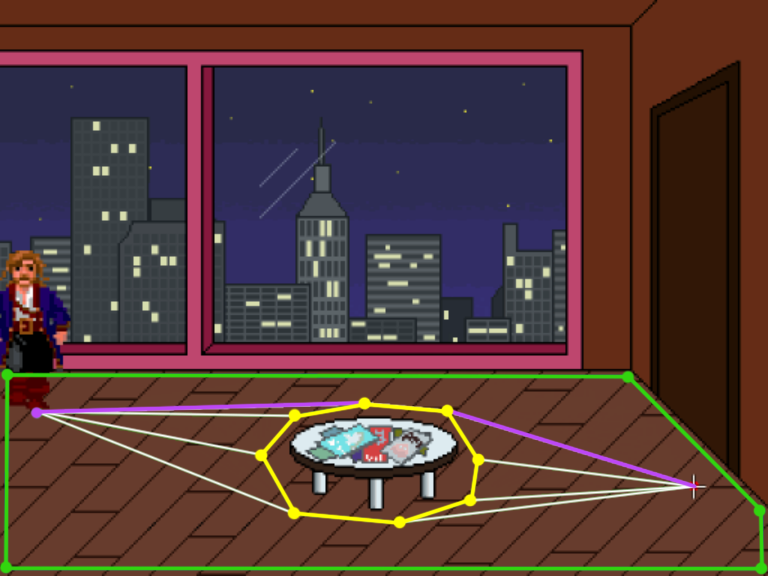
\includegraphics[width=.7\linewidth]{img/WS-polygons3.png}
\caption{Graph: Walkable area consisting of polygons (green and yellow) and a graph (white) with a possible path (violet). Source \cite{Uurloon1}.}
\label{fig:Graph}
\end{figure}

\subsubsection{A* algorithm}
When it comes to choosing a pathfinding algorithm, our goal is to find one that reliably and efficiently determines the shortest path between two points in a 2D space. Since our maps typically contain only a few dozen vertices, raw performance is not a critical concern. Among the most commonly used algorithms in game development is A*, known for its balance of simplicity and efficiency. While our project doesn’t demand high performance, A* still meets all our needs and is straightforward to implement. Moreover, if the project were to scale and require handling more complex maps with a larger number of vertices, A* would still be a solid choice due to its proven performance. 

A key component of the A* algorithm is the heuristic function which estimates the cost of the cheapest path to the goal. If the function never overestimates it, A* is guaranteed to return one of the shortest paths from start to goal. For the purpose of free character movement on a 2D plane, the Euclidean distance was chosen as a heuristic function. It is well suited for point-and-click adventure games, where characters can move freely in any direction, making straight-line distance a natural and accurate estimate of travel cost.  It can be calculated from the Cartesian coordinates of the points while also applying the Pythagorean theorem:

\[
d = \sqrt{(x_2 - x_1)^2 + (y_2 - y_1)^2}
\]

\section{Depth Simulation}
As we have specified in Requirements \ref{intro:req:scale} and \ref{intro:req:layers}, we want to simulate the feeling of a 3D space. 

\subsection{Scaling}
\label{analysis:depth:scaling}
The human eye perceives depth by observing objects in the distance as smaller than they actually are. There are a number of ways we can simulate this phenomenon in a 2D video game. One option would be to scale the size of the character based only on the Y coordinates. This way, we can set the boundaries for the minimum and maximum scale of the moving object in the given area, and then, based on the distance from those boundaries, set the appropriate value, visualized in Figure \ref{fig:Room} . This approach is very simple, which is both its advantage and its disadvantage. Although it is easy to implement, it is not possible to achieve more complex scenes in which a character's sprite scales dynamically independently of the Y coordinates. A similar problem would arise with only considering the X coordinates.


\begin{figure}[H]
\centering
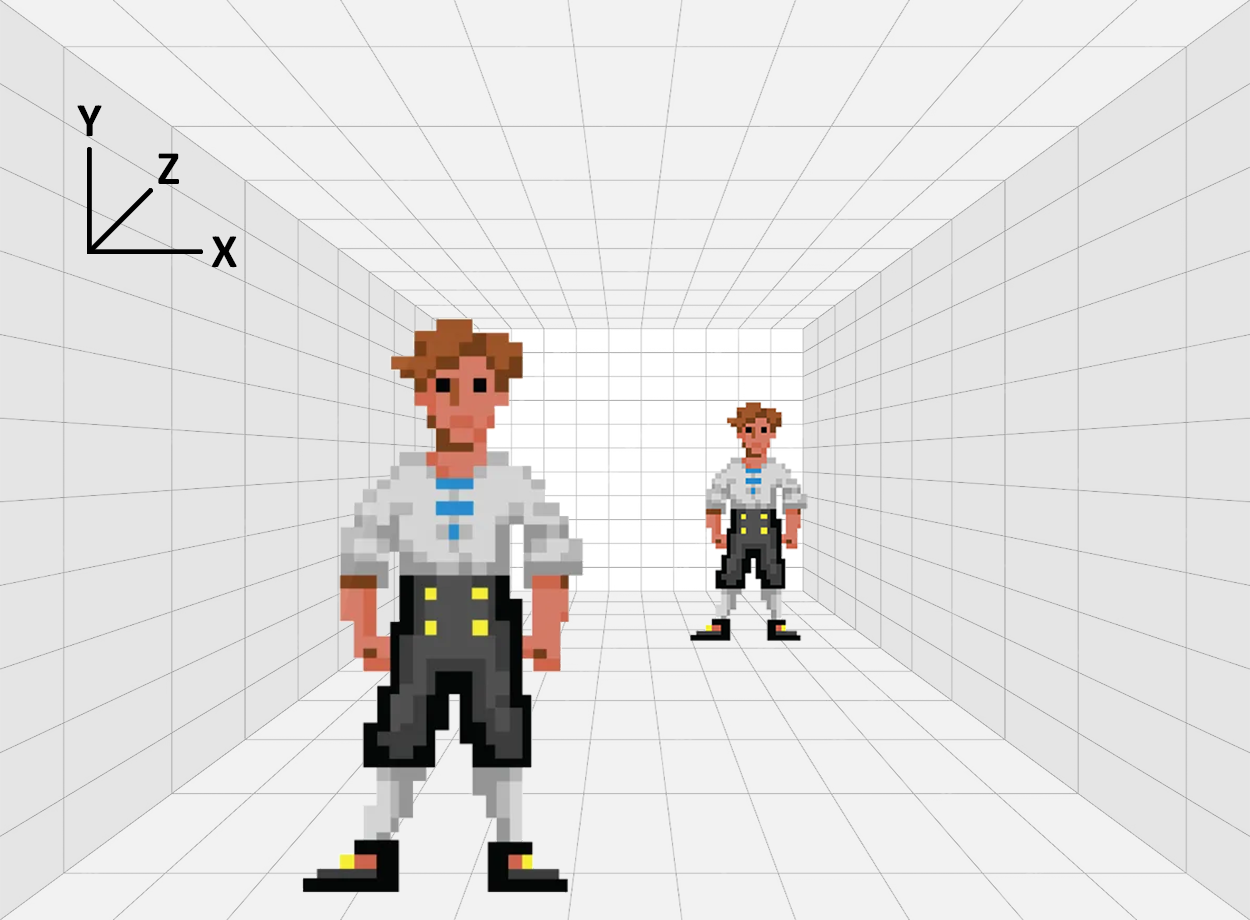
\includegraphics[width=.6\linewidth]{img/room.png}
\caption{Character scaling by Y axis.}
\label{fig:Room}
\end{figure}

Our goal is to dynamically scale the character sprite based on its position on the map. To achieve this, we need a system that adjusts the sprite’s size depending on its location. A suitable way to store this scaling data is by assigning it to the vertices of the polygons that define the walkable area. Each vertex could carry a floating-point value representing the desired scale at that point, allowing us to interpolate the character's size as it moves across the map.  An advantage is the fact that the developer could have a free range on the exact details of the area. However, modifying the scales is not that easy because one must go through the necessary nodes and change the factor essentially by hand. This approach is a bit more complicated than the previous ones, but still fairly simple to implement and doable entirely in Unity.

Finally, it is possible to use a bitmap and map the alpha value of each pixel to a scaling factor. This would be very precise, as the developer can set it up exactly as they wish. However, we again come across the problem we discussed in Section \ref{analysis:walkableMap} where we made it clear that we prefer to implement features that can be simply modified inside Unity.

From these three approaches only two seem to be doable entirely inside the framework: Y scaling (optionally X scaling) and custom vertices scaling. We aim to implement both of them in the hopes of offering a wide variety of options to developers.

\subsection{Layering}
Next, let us examine the layering. Our aim is to dynamically adjust the visibility of objects, as seen in Figure \ref{fig:Layers}. The human eye and brain can process this kind of information in the real world naturally and can therefore create a visual image of how objects are ordered one after the other. Because we are working with a 2D space, we have to do a bit more work simulating this phenomenon and determining in what order the sprites of objects should be displayed. Fortunately, it is very simple since all we need is to look at the Y coordinates. If object A has a smaller Y coordinate than object B, it means that A should be drawn on top of B. This is not complicated, but also not trivial, since it would be necessary to perform this check between each two objects in the scene. Lucky for us, Unity offers tools for 2D renderer sorting \cite{Unity-sorting} and can therefore take care of this problem for us. What we are looking for is the Custom Axis sort mode \cite{Unity-customAxis} in Graphics section under the Project Settings window. Details on the setup with a couple more modifications to make it just right can be found online in the Sunny Valley Studio article \cite{Piotr} . 

\begin{figure}[H]
\centering
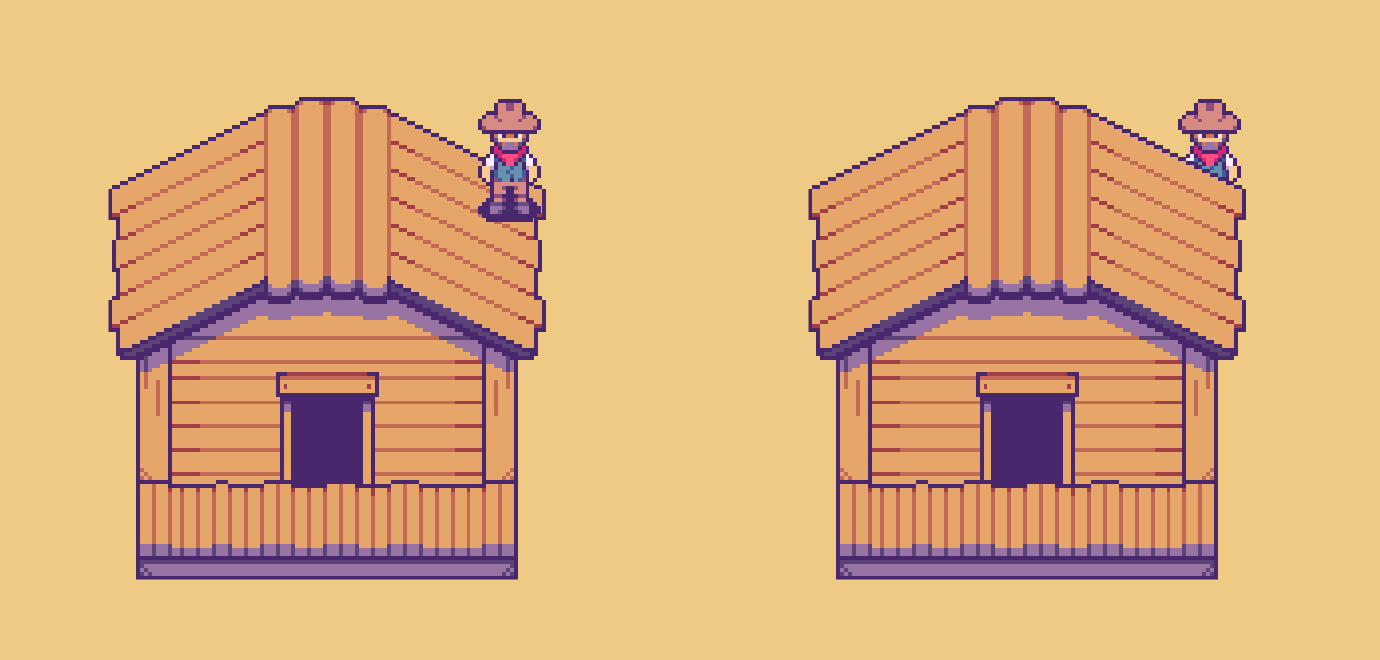
\includegraphics[width=.8\linewidth]{img/layers.png}
\caption{Wrong (left) and correct (right) 2D layer ordering. Source \cite{Piotr}.}
\label{fig:Layers}
\end{figure}

\section{Inventory System}


\section{Dialogue System}
Conversations between characters help players understand the story and connect with the game world. While they usually take the form of a dialogue between two characters, that is not always the case. When only one character is speaking, it becomes a monologue or thinking aloud. On the other hand, conversations can also involve more than two characters, resulting in group interactions. 

In cases where dialogue is limited to a simple exchange of lines without requiring player input, the representation of a conversation can be fairly straightforward: the dialogue can be stored as a list of data containing the text and other relevant information. In an \textit{Game Dev Beginner} article \cite{Dialogue-French}, John French presents a possible implementation of this approach.  However, this linear method has its drawbacks. Managing longer conversations can become cumbersome as one needs to scroll through the entire list to reach specific lines, which quickly becomes inconvenient. The situation becomes even more complex when players are given the ability to make choices. Even a handful of branching lines can lead to a complicated structure that is nearly impossible to manage using a linear format. The complexity increases further when cyclic paths are introduced, where characters may repeat lines in response to specific prompts. Implementing such behavior in a linear format is not only difficult, but also tends to produce a cluttered and confusing system. 

Due to the limitations of the linear method, it is necessary to explore more flexible solutions. A particular data structure that can effectively represent the complexity of a branching dialogue is a graph. Its structure allows for direct access to specific dialogue lines and, in the case of branching paths, offers an intuitive way to manage and visualize the flow. Additionally, graphs make it easy to implement cyclic paths, enabling characters to reuse parts of the dialogue under certain conditions. Looking at these advantages, it is clear that this data structure is suitable for our needs. So, let us take a look at the tools Unity offers for creating graphs.

\subsection{Graph Tools in Unity}
Currently, there is no officially supported non-experimental graph tool or framework available in Unity. A new system named \textit{Graph Toolkit}  \cite{Unity-GraphToolkit} is under development and aims to provide a unified solution for graph-based editing. However, it has not yet been released. Due to the lack of official support, alternative options must be explored. Since one of the core goals of this project is to remain free and open source, the tools used should ideally follow the same principles. While the Unity Asset Store offers numerous graph-based tools, many of them do not meet these criteria. Tools such as \textit{FlowCanvas} \cite{FlowCanvas}, \textit{Xtebs Graph Framework} \cite{XtebsGraphFramework}, and \textit{uNode 3 Pro} \cite{uNode3Pro} are all commercial products. On the other hand, \textit{FlowReactor} \cite{FlowReactor} and \textit{xNode} \cite{xNode} are free but have not received updates in several years. \textit{NodeGraphProcessor} \cite{NodeGraphProcessor} emerged as a potential candidate, but its complexity and extensive set of features go beyond the needs of this project.

Among the tools offered directly by Unity, we identified \textit{GraphView} \cite{Unity-GraphView} as a possible solution. It is a C\# API provided through Unity’s UI Toolkit framework, designed for building custom, node-based editor tools within Unity Editor. GraphView is commonly used in the creation of visual scripting environments, dialogue systems, shader editors, behavior trees, and similar graph-based tools. However, it remains experimental and lacks official documentation, as it is within the \verb|UnityEditor.Experimental.GraphView| namespace. Notably, NodeGraphProcessor itself is built on top of GraphView, highlighting its utility despite its unofficial status.

Although the current state of graph tool support in Unity is somewhat fragmented, we ultimately decided to build a custom graph system using GraphView. Despite its limitations, GraphView continues to enjoy community interest, with recent tutorials drawing significant attention \cite{NodeEditor-YT}. Moreover, it remains supported in Unity 6, ensuring that it will remain viable for at least the near future—until the release and widespread adoption of the upcoming Graph Toolkit.

For the implementation of the dialogue system, we plan to follow the approach developed by \textit{Kasper Dev Unity}, who created a project \cite{Kasper-Dialogue-Tutorial-git} and a series of tutorials \cite{Kasper-Dialogue-Tutorial-YT} focused on building a dialogue system using Unity’s GraphView API. His method offers a clear and practical foundation for creating node-based dialogue editors, which fits well with the goals of this thesis. While his work will serve as the main reference, we also want to explore other tutorials, such as those by \textit{Mert Kirimgeri} \cite{merpheus-Dialogue-Tutorial-git}\cite{merpheus-Dialogue-Tutorial-YT} and \textit{Indie Wafflus} \cite{Wafflus-Dialogue-Tutorial-git}\cite{Wafflus-Dialogue-Tutorial-YT}—to gather different ideas and perspectives. By combining the strengths of these approaches, we aim to build a system that is well-suited to the needs of this project: flexible enough to handle branching and cyclic dialogue, but still simple and intuitive for developers to use. 